\chapter{Graph Convolutional Neural Network}
\section{Definition}
\paragraph{} Graph Convolutional Network (GCN) is a semi-supervised learning algorithm for graph-structured data. This is
refered convolutional, because filter parameters are typically shared over all locations in the graph.
\paragraph{} GCN model goal is to learn a function of signals/features on a graph $G=(V,E)$
which takes input:
\begin{itemize}
    \item A feature description $x_i$ for every node $i$,summarized in a $N \times D$.
    \item A representative description of the graph structure in matrix form; typically in the form of an adjacency matrix $A$.
\end{itemize}
\paragraph{} It produces node level output $Z$ (an $N \times F$), where $F$ is the 
number of output features per-node.
\section{GCN mathematical formulation}
\paragraph{} A simple neural l-th layer network as per above definition can be formulated as
\begin{equation}
    f(H^l,A) = \sigma(A H^l W^l)
\end{equation}
\paragraph{} The main limitation on the above formulation is $A$ is not normalized therefore 
the multiplication with $A$ will completely change the scale of the feature vectors. The adjacency
matrix can be normalized (making row sum equal to 1) by multiplying inverse of the diagonal matrix with has
degree value of each node in the diagonal($D$)(i.e $D^{-1}A$)
\paragraph{} The mathematical fomulation of GCN as follows:
\begin{equation}
    f(H^l,A) = \sigma(\hat{D}^{-\frac{1}{2}} \hat{A} \hat{D}^{\frac{1}{2}} H^l W^l)
\end{equation}
\paragraph{} where $\hat{A} = A+I$ is the adjacency matirx after adding self loop and $I$ is the identity matrix,
$\hat{D}^{-\frac{1}{2}} \hat{A} \hat{D}^{\frac{1}{2}}$ is the symmetric normalization for better convergence rather than 
normal normalization and $\sigma$ is the non-linear activation functon.
\section{GCN pictorial representation}
\begin{figure}[h]
    \centering
    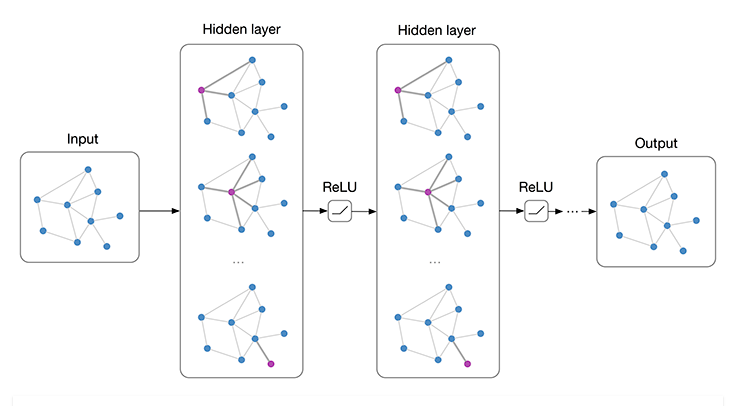
\includegraphics[width=10cm,height=5cm]{tex/img/GCN.png}
    \caption{multi-layer GCN network}
\end{figure}
\paragraph{} The above figure 5.1 represents the pictorial representation of multi-layer GCN with one hidden layer.
At each layer the model learns the node features with respect to grap structure and the node's inherient features.